
%(BEGIN_QUESTION)
% Copyright 2005, Tony R. Kuphaldt, released under the Creative Commons Attribution License (v 1.0)
% This means you may do almost anything with this work of mine, so long as you give me proper credit

Noen av følgende transistorsvitsjekretser er riktig koblet, og noen er ikke. Identifiser hvilke kretser som fungerer riktig (dvs. slår på lasten når bryteren lukkes), og hvilke som er feilkoblet:

$$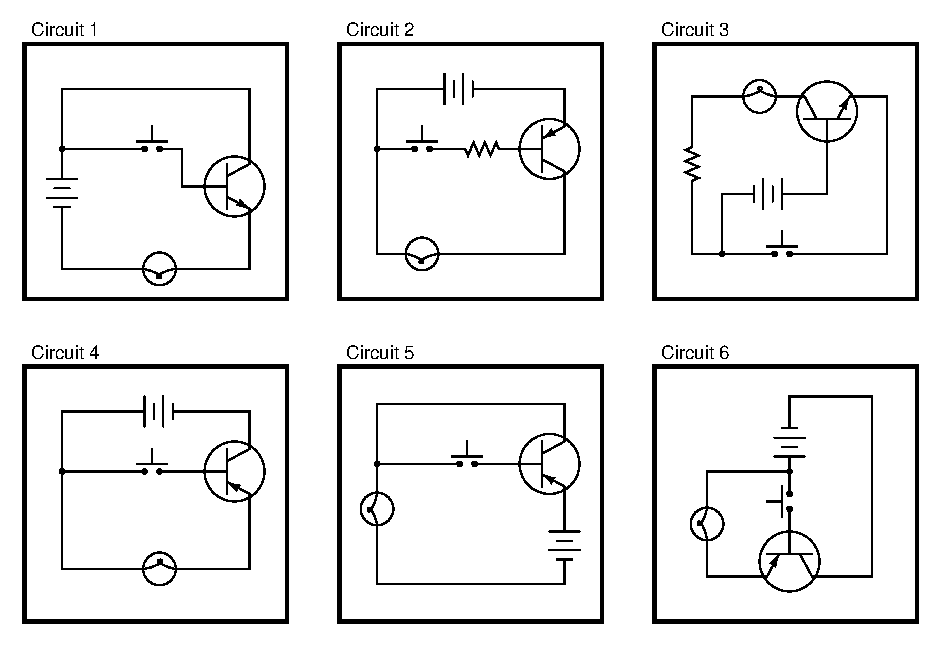
\includegraphics[width=15.5cm]{i01004x01.eps}$$

\underbar{file i01004}
%(END_QUESTION)





%(BEGIN_ANSWER)

Husk at en bipolar transistor krever strøm gjennom base-emitter-overgangen for å slå inn, slik at laststrøm kan gå mellom kollektor og emitter.

$$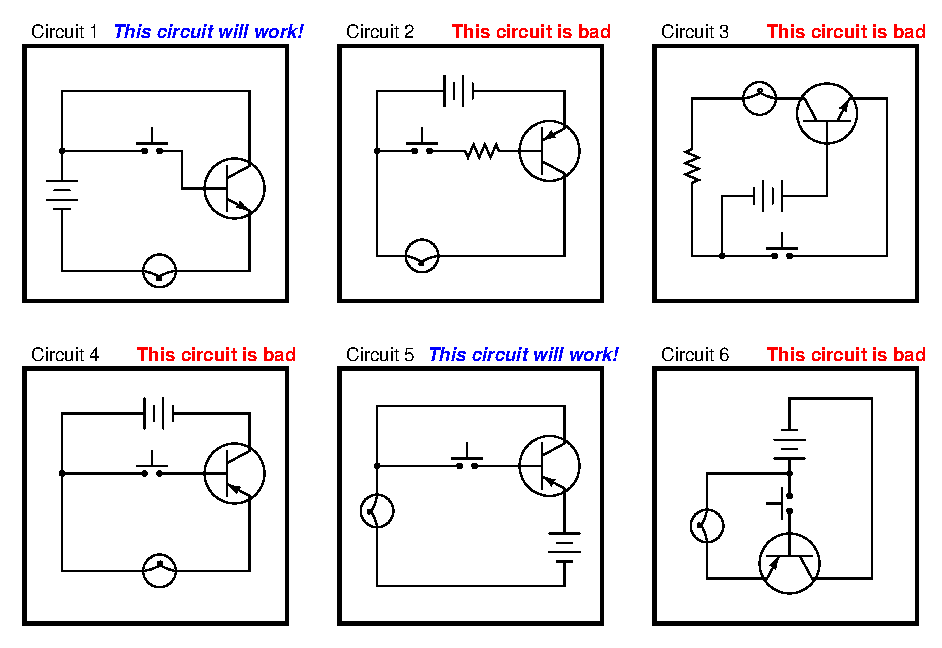
\includegraphics[width=15.5cm]{i01004x02.eps}$$

\vskip 10pt

Krets \#3 er annerledes enn de andre ``dårlige'' kretsene: lampen i krets \#3 lyser svakt når trykknappen er åpen, fordi strøm kan gå gjennom base-kollektor-overgangen som gjennom en diode.

%(END_ANSWER)





%(BEGIN_NOTES)


\vskip 20pt \vbox{\hrule \hbox{\strut \vrule{} {\bf Virtuell feilsøking} \vrule} \hrule}

Denne oppgaven egner seg godt som feilsøkingsøvelse der man simulerer symptomer og tester.

\begin{itemize}
\item{} Hva forteller resultatet av siste test om feilen?
\item{} Hvis siste test ga et annet resultat, hva ville det betydd?
\item{} Var siste test den beste mulige testen?
\item{} Hva er ideell testrekkefølge for færrest mulige steg?
\end{itemize}

%INDEX% Electronics review, transistor switch circuit (BJT)

%(END_NOTES)

